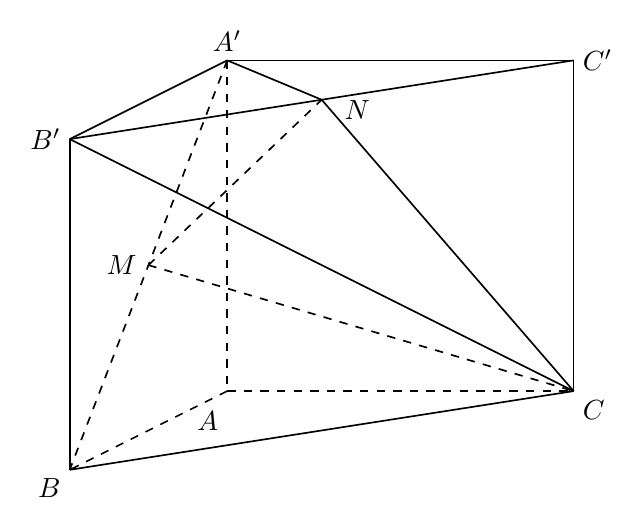
\begin{tikzpicture}[x=1cm,y=1cm,line width=.6pt,font=\normalsize]
\tikzset{ptlabel/.style={fill=none,inner sep=1pt,font=\normalsize}}
\coordinate (Ap) at (2.6,5.2);
\coordinate (Cp) at (7,5.2);
\coordinate (Bp) at (0.6,4.2);
\coordinate (A) at (2.6,1.0);
\coordinate (C) at (7.0,1.0);
\coordinate (B) at (0.6,0.0);
\coordinate (M) at (1.6,2.6);
\coordinate (N) at (3.8,4.7);
% top triangle
\draw (Ap) -- (Cp);
\draw (Ap) -- (Bp);
\draw (Bp) -- (N) -- (Cp);
% verticals: B'B solid per original science figure
\draw[dashed] (Ap) -- (A);
\draw (Bp) -- (B);
\draw (Cp) -- (C);
% bottom triangle
\draw[dashed] (A) -- (C);
\draw[dashed] (A) -- (B);
\draw (B) -- (C);
% diagonals
\draw[dashed] (Ap) -- (B);
\draw (Bp) -- (C);
\draw (Ap) -- (N);
\draw (N) -- (C);
% interior dashed
\draw[dashed] (M) -- (N);
\draw[dashed] (M) -- (C);
% labels
\node[ptlabel,above=2pt] at (Ap) {$A'$};
\node[ptlabel,right=2pt] at (Cp) {$C'$};
\node[ptlabel,left=2pt] at (Bp) {$B'$};
\node[ptlabel,below left=2pt,xshift=0.00bp,yshift=-4.00bp] at (A) {$A$};
\node[ptlabel,below right=2pt] at (C) {$C$};
\node[ptlabel,below left=2pt] at (B) {$B$};
\node[ptlabel,left=3pt] at (M) {$M$};
\node[ptlabel,below right=1pt,xshift=6.00bp,yshift=2.00bp] at (N) {$N$};
\end{tikzpicture}
